% run the command ' lualatex -shell-escape Reference.tex ' twice in the terminal to visualize table of contents
\documentclass[twoside]{article}
\usepackage[utf8]{inputenc}
\usepackage[spanish]{babel}
\usepackage{geometry}
\usepackage{multicol}
\usepackage{minted}
\usepackage{python}
\usepackage[hidelinks]{hyperref}
\usepackage{fancyhdr}
\usepackage{listings}
\usepackage{pdfpages}
\usepackage{needspace}
\usepackage{sectsty}
\usepackage{array}
\usepackage{multirow} 
\usepackage{longtable}
\usepackage{xcolor}
\usepackage{afterpage}
\usepackage{amssymb}
\usepackage{amsmath}
\usepackage[inline]{enumitem}
\usepackage{graphicx}


\newcommand{\wdir}[1]{/home/san/Algorithms/Reference/#1}
\geometry{letterpaper, portrait, left=0.5cm, right=0.5cm, top=1.8cm, bottom=1cm}

\sectionfont{\Huge\bfseries\sffamily}

\definecolor{LightGray}{gray}{0.9}
\definecolor{prussianblue}{rgb}{0.0, 0.19, 0.33}
\definecolor{indigo(dye)}{rgb}{0.0, 0.25, 0.42}
\definecolor{lapislazuli}{rgb}{0.15, 0.38, 0.61}
\definecolor{mediumelectricblue}{rgb}{0.01, 0.31, 0.59}
\definecolor{smalt(darkpowderblue)}{rgb}{0.0, 0.2, 0.6}
\definecolor{yaleblue}{rgb}{0.06, 0.3, 0.57}
\definecolor{skobeloff}{rgb}{0.0, 0.48, 0.45}
\definecolor{pinegreen}{rgb}{0.0, 0.47, 0.44}

\setminted{
    style=tango,
    breaklines=true,
    bgcolor=LightGray
}

\setlength{\headsep}{0.5cm}
\setlength{\columnsep}{0.5cm}
\setlength{\columnseprule}{0.01cm}
\renewcommand{\columnseprulecolor}{\color{gray}}

\pagestyle{fancy}
\pagenumbering{arabic}
\fancyhead{}
\fancyfoot{}
\fancyhead[LO,RE]{\textsf{First, solve the problem. Then, write the code.}}
\fancyhead[LE,RO]{\textsf{\leftmark}}
\fancyfoot[LE,RO]{\textbf{\textsf{\thepage}}}
 
\renewcommand{\headrulewidth}{0.01cm}
\renewcommand{\footrulewidth}{0.01cm}

\setlength{\parindent}{0em}
% column space
\setlength{\tabcolsep}{10pt} % Default value: 6pt
% upper and lower padding
\renewcommand{\arraystretch}{1.5} % Default value: 1

\begin{document}
\null
\thispagestyle{empty}
\newpage
\fontfamily{lmss}
\selectfont
\tableofcontents
\newpage
\cleardoublepage
\section{Introduccion a las bases de datos}

\section{Conceptos de sistemas y arquitectura de bases de datos}

\subsection{Concepto de Base de datos}

Una base de datos se puede definir como un conjunto de datos ''ordenados'', definidos por un modelo de datos, los cuales se almacenan en dispositivos de almacenamiento.\\

Su finalidad es: Manipular, controlar, consultar, preservar los datos de la misma.

\subsection{Sistemas de Base de Datos} % **********************PENDIENTE DE PREGUNTAR A QUE SE REFIERE*************************
\subsection{Aplicaciones de los Sistemas de BD}

\subsection{Proposito de los sistemas de BD}

Los sistemas de bases de datos tienen como intencion solucionar los problemas que se derivan de utilizar un sistema meramente de archivos.
Algunos de estos problemas son:

\begin{itemize}
  \item Los datos aparecen de manera redundante.
  \item Los datos son inconsistentes.
  \item Los datos se encuentran totalmente aislados.
  \item No es posible el acceso concurrente
\end{itemize}

En cambio, los Sistemas de Bases de Datos cumplen con las siguientes caracteristicas:

\begin{itemize}
  \item Minimizan la redundancia en los datos.
  \item Eliminan inconsistencias en los datos.
  \item Permiten la comunicacion con distintos repositorios de datos.
  \item Mantiene un control de concurrencia en las transacciones.
\end{itemize}

[Nota]\\
Una transaccion es una operacion que afecta al Repositorio de datos, pueden ser de diferentes tipos como:\\
\begin{itemize}
  \item Insercion
  \item Actualizacion
  \item Eliminacion
  \item Consulta
\end{itemize}


\subsection{Usuarios de la BD}

\subsubsection{Administrador de BD}

Encargado de:

\begin{itemize}
  \item Monitarear el performance.
  \item Define tiempos de respaldo.
  \item Proceso de tunning \rightarrow afinacion / reorganizacion fisica.
  \item Llevar a cabo las tecnicas de recuperacion.
  \item Administra herramientas [Objetos accedidos, Matriz de autorizacion: creacion de cuentas de usuarios]
\end{itemize}

\subsubsection{Diseñadores de la BD}

\begin{itemize}
  \item Genera propios modelos de datos [conceptuales (E/R), logicos (Relacionales), fisicos (Indices)]
  \item Genera esquema de BD: [Medicas, Administrativas, Puntos de esquema]
\end{itemize}

----------Inserte aqui diagramas de ejemplo para modelos conceptuales y logicos.---------------

\subsubsection{Programadores de aplicaciones}

\begin{itemize}
  \item Interfaces de los usuarios finales (Dashboards) (facilita el acceso a "ciertos" objetos de la BD)
  \item Interfaces para la gestion de aplicaciones.
  \begin{itemize}
    \item IDE's (java / .NET)
    \item Lenguajes scripts
    \item Conectividad con el servidor de datos (APIs)
    \item Programacion Orienteada a Objetos
  \end{itemize}
\end{itemize}

\subsubsection{Usuarios Finales}

\begin{itemize}
  \item Usuarios casuales (nivel gerencia)
  \begin{itemize}
    \item Inteligencia (Big Data)
    \item Negocios
    \item Reportes (Toma de decisiones)
  \end{itemize}
  \item Principales o parametricos
  \begin{itemize}
    \item Puntos de ventas
  \end{itemize}
  \item Sofisticados
  \begin{itemize}
    \item Desarrolladores de apps
    \item DBAs (Admins de Bases de Datos)
    \item Investigadores
  \end{itemize}
  \item Independientes (Stand Alone)
  \begin{itemize}
    \item Proyectos Escolares
    \item No hay conectividad con otros "nodos" a la internet
  \end{itemize}
\end{itemize}

\subsection{Ciclo de vida de una BD}

\begin{enumerate}
  \item Planificacion
  \begin{itemize}
    \item Viabilidad de la implementacion
    \item Supervisores, dueños, gerentes
    \item Contexto, ¿ Para que ?, citas, control, etc.
    \item Tiempos de entrega
  \end{itemize}
  \item Analisis y Formulacion de Requerimientos (Acciones que debe hacer nuestro sistema)
  \begin{itemize}
    \item Contexto
    \item Requerimientos [Basicos, Funcionales, No Funcionales]
    \item Reglas del negocio (Proceso) \rightarrow restricciones (IDE's)
  \end{itemize}
  \item {Diseño}
  \begin{itemize}
    \item Generar los modelos de datos [logicos, conceptuales y fisicos] orientados a objetos relacionales, multidimensionales.
    \item Aplicaciones de usuarios finales (Diseñar GUI) \rightarrow HCI (Human Computer Interaction)
  \end{itemize}
  \item Implementacion
  \begin{itemize}
    \item Construir el repositorio de datos
    \item Conectar al servidor
  \end{itemize}
  \item Operacion y Mantenimiento
  \begin{itemize}
    \item Crecimiento de usuarios y datos
    \item Posibles cambios que se deban realizar
    \item Errores y Correcciones
    \item Monitoreo
  \end{itemize}
\end{enumerate}

\subsection{Modelos de de datos}



\subsubsection{Conceptual}

\begin{itemize}
  \item Permiten definir el ambito / context de la BD
  \item Lenguaje natural (idioma nativo)
  \item Comprendido por cualquier persona
  \item Proceso de analisis de requerimientos
  \item Diagrama Entidad / Relacion o Entidad / Asociacion
\end{itemize}

--------------------Inserte ejemplo de Esquema Conceptual-------------------

\subsubsection{Logico}

\begin{itemize}
  \item Definen el esquema de base de datos en terminos de relacion
  \item Tablas:
  \begin{itemize}
    \item Filas (tuplas)
    \item Columnas (nombre \rightarrow atributo)
    \item claves relacionales [Primary Key, Foreign Key, Candidate key]
    \item Tipos de datos
    \item Constraints (restricciones)
  \end{itemize}
  \item Puedes construir la BD fisicamente
  \begin{itemize}
    \item Manual
    \item Automatica (Herramientas CASE)
  \end{itemize}
\end{itemize}

------------------Inserte ejemplo de Esquema Logico--------------------

\subsubsection{Fisico}

Depende del Sistema Operativo

\begin{itemize}
  \item Define las estructuras de almacenamiento de datos.
  \item Define los indices(index) para acceder a los archivos fisicos del repositorio de datos.
\end{itemize}

-----------------Inserte ejemplo de Esquema Fisico----------------------


\subsection{Arquitectura de 3 niveles}

\subsubsection{Nivel externo}

Describe una parte de la BD que es relevante a un usuario en particular, excluye datos irrelevantes asi como informacion a la que el usuario
no se le tiene permitido el acceso.

Los usuarios finales son quienes visualizan este nivel por medio de GUIs.

\subsubsection{Nivel conceptual}

Describe:

\begin{itemize}
  \item Que datos se almacenan.
  \item Como se relacionan los datos entre ellos.
\end{itemize}

Algunas de sus caracteristicas son:

\begin{itemize}
  \item El DBA trabaja en este nivel.
  \item Describe la estructura de todos los usuarios.
  \item Solo el DBA define este nivel.
  \item Da una vista global de la BD.
  \item Es independiente del software y hardware.
\end{itemize}

\subsubsection{Nivel interno}

Describe como la informacion es almacenada en la BD.

\begin{itemize}
  \item Define las estructuras de almacenamiento (depende del S.O.)
  \item Define la construccion
\end{itemize}

\subsection{Independencia de datos}

\begin{itemize}
  \item \textbf{Independencia Logica:} Capacidad de modificar el esquema conceptual sin tener que alterar los esquemas externos ni los programas de aplicacion.
  \item \textbf{Independencia Fisica:} Capacidad de modificar el esquema interno sin tener que alterar el esquema conceptual (o los externos).
\end{itemize}

\subsection{Arquitectura de los SGBD}

\begin{enumerate}
  \item Aplicaciones de usuarios finales
  \item Comandos SQL
  \item SGBD
  \begin{enumerate}
    \item Motor de evaluacion de consultas
    \begin{enumerate}
      \item Analizador
      \item Evaluador de Operadores
      \item Optimizador
      \item Ejecutor de planes
    \end{enumerate}
    \item Control de concurrencia
    \item Archivos
    \begin{itemize}
      \item Catalogo del sistema
      \item Archivo de indices
      \item Archivos de datos
    \end{itemize}
  \end{enumerate}
\end{enumerate}

\begin{figure}[~htb]
  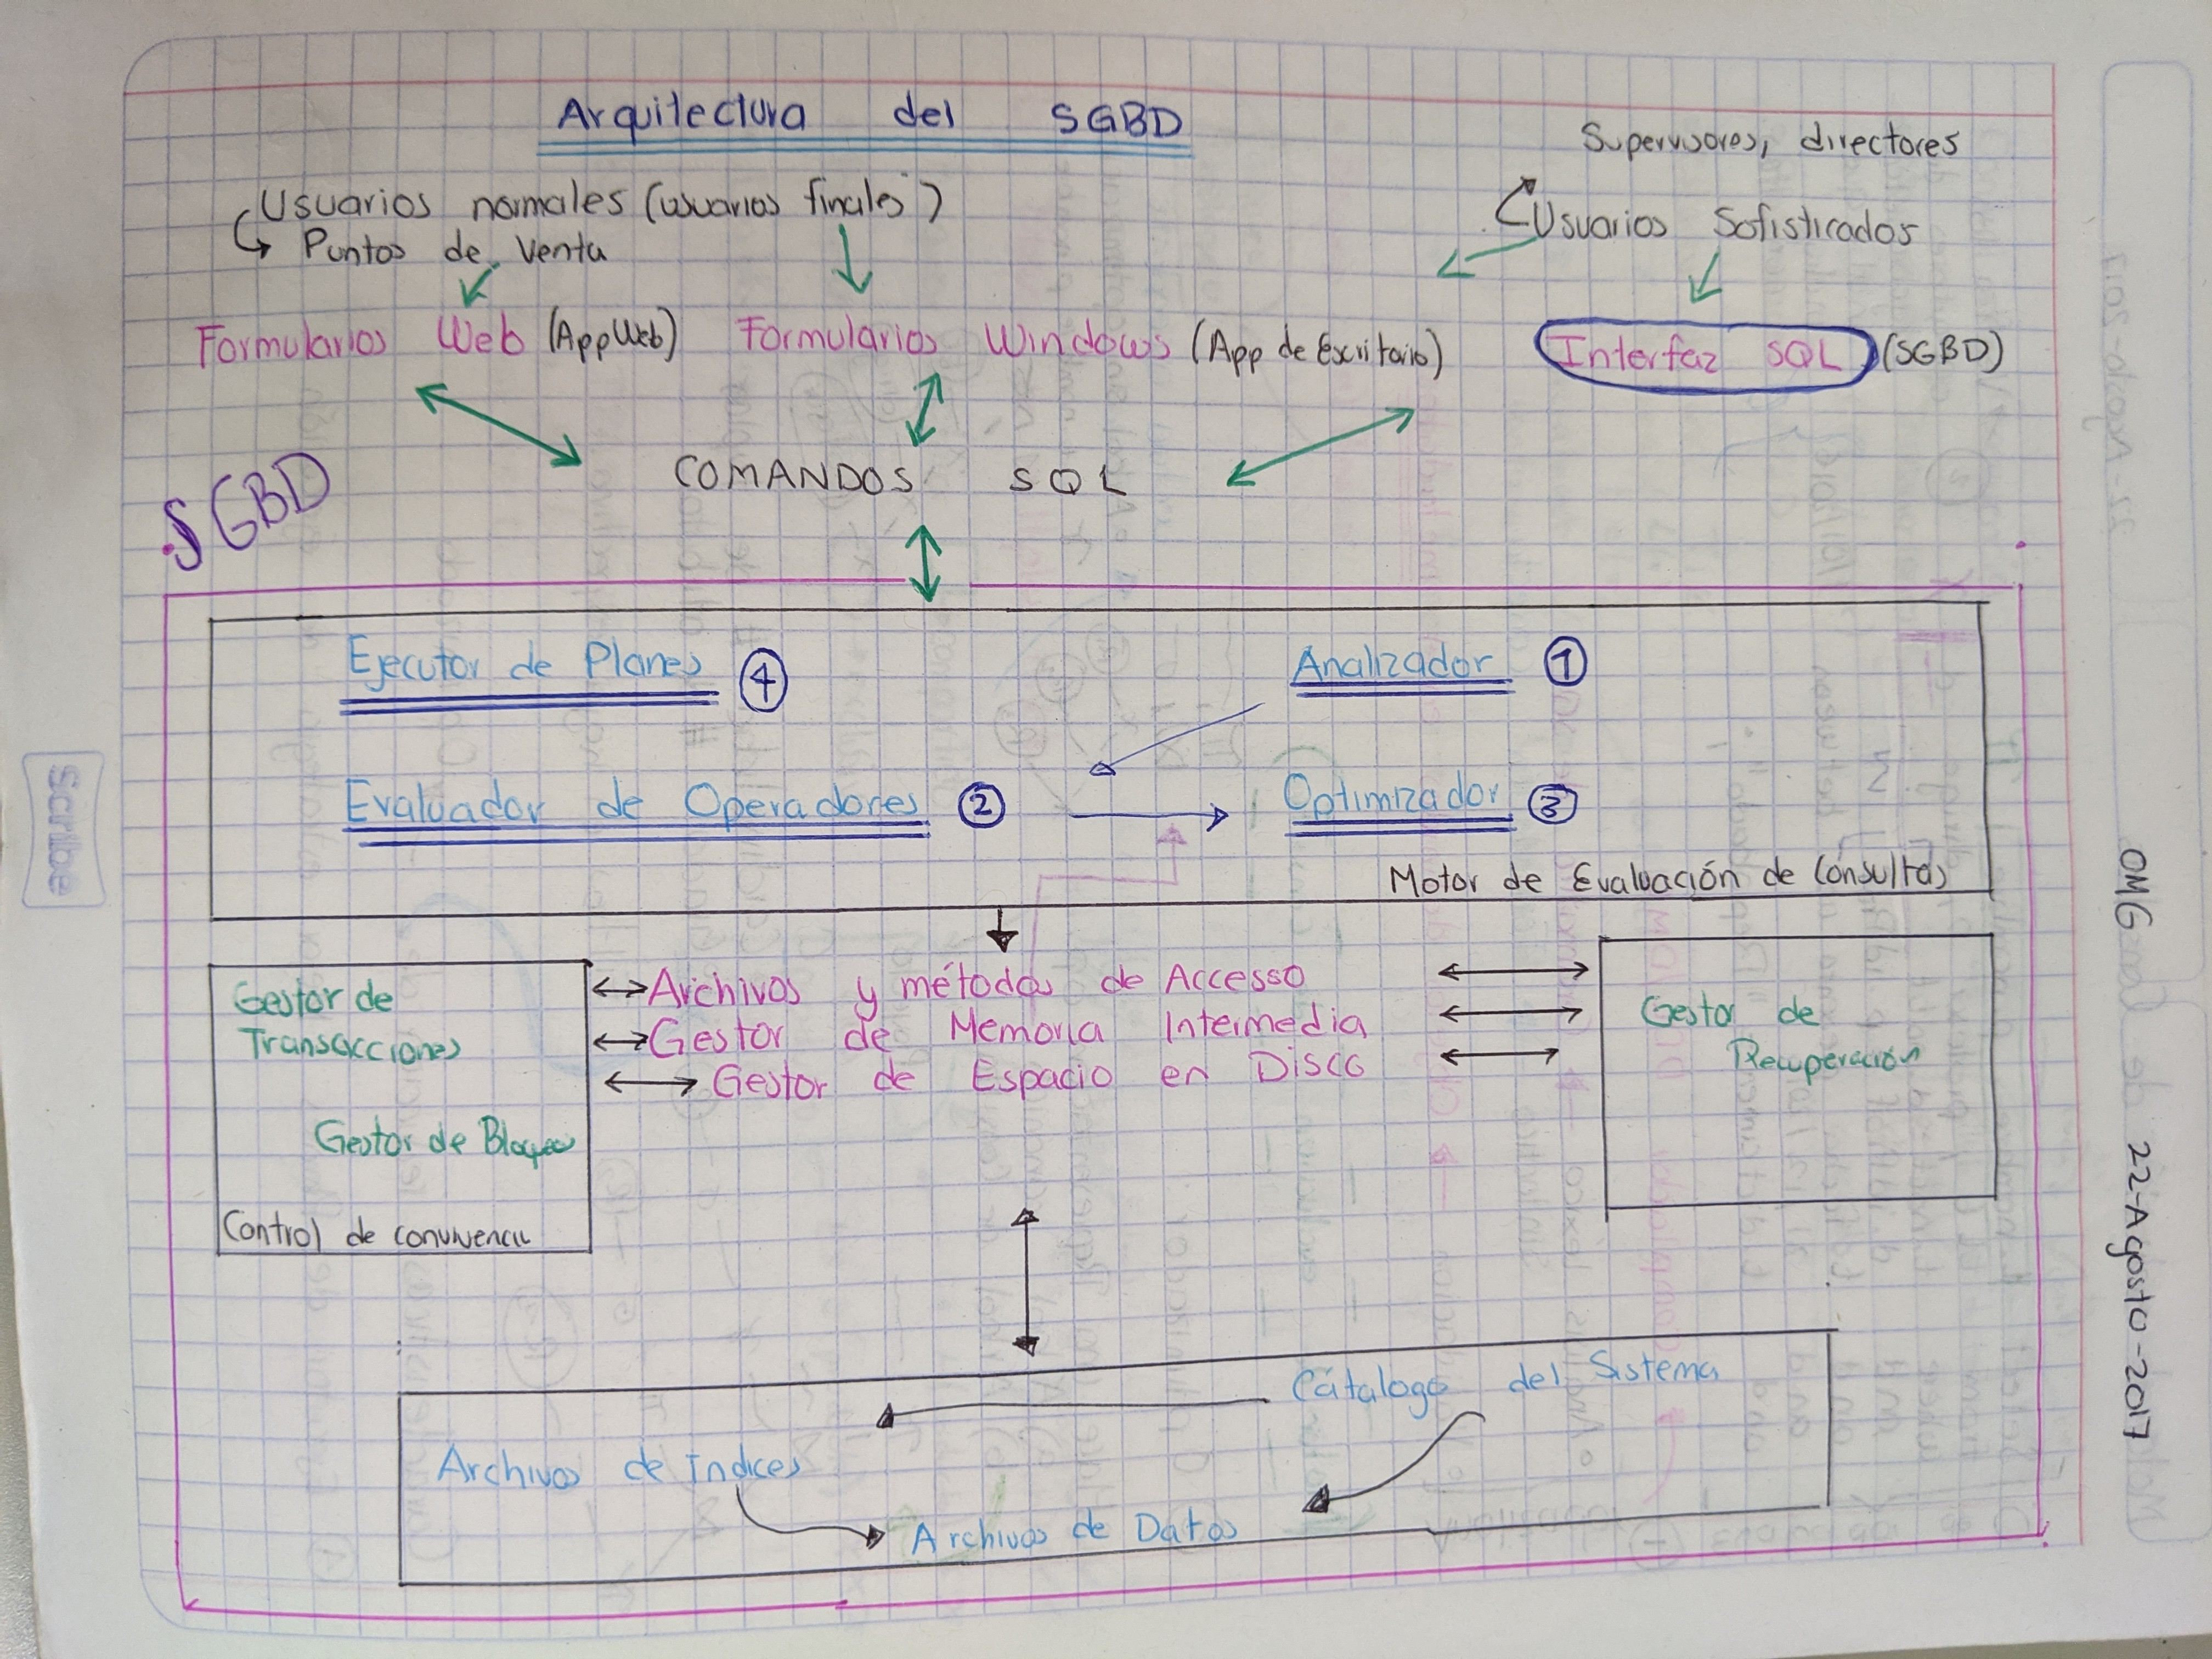
\includegraphics[width=\linewidth]{arqsgbd.jpg}
  \caption{Arquitectura de un SGBD}
\end{figure}

\clearpage

\subsection{DDL Data Definition Language}
Involves:
\begin{itemize}
	\item create table
	\item drop table
\end{itemize}

\subsection{DML Data Manipulation Language}
Involves:
\begin{itemize}
	\item insert into
	\item delete
	\item select
	\item update
\end{itemize}
\section{Algebra relacional y SQL standar}
\textbf{DEF.} Una expresion en el algebra relacional se construye a partir de subexpresiones.\\

Sean $E_1$ \& $E_2$ expresiones del algebra relacional. Las siguientes son todas expresiones \textbf{binarias} del algebra relaional.\\

\begin{itemize}
  \item \textbf{Union:} $E_1 \cup E_2$ (Se requiere que el numero de columnas sea el mismo entre tablas asi como los nombres de columnas.)
  \item \textbf{Diferencia:} $E_1 - E_2$
  \item \textbf{Producto Cartesiano:} $E_1 \times E_2$
\end{itemize}

Y las siguientes son operaciones \textbf{unarias:}\\

\begin{itemize}
  \item \textbf{Seleccion:} $\sigma_p(E_1)$ donde $p$ es un predicado de atributos de $E_1$. (Trabaja con renglones completos)\\
  \item \textbf{Proyeccion:} $\Pi_s(E_1)$ donde $s$ es un conjunto de atributos de $E_1$. (Trabaja con columnas completas)\\
  \item \textbf{Renombramiento:} $P_x(E_1)$ donde $E_x$ es un nuevo nombre de la relacion $E_1$.
\end{itemize}

\newpage

Sean $R$, $S$ y $T$ entidades ejemplificaremos las operaciones mencionadas anteriormente:\\
\begin{center}
\begin{tabular}{ccc}
\multicolumn{3}{c}{\textbf{Entidades}}
\tabularnewline
\begin{minipage}{.25\linewidth}
\begin{tabular}{| >{\centering}m{1cm}| >{\centering}m{1cm}| >{\centering}m{1cm}|}
\hline
\multicolumn{3}{|c|}{\textbf{R}}
\tabularnewline \hline
\textbf{A}
&
\textbf{B}
&
\textbf{C}
\tabularnewline \hline
a & 1 & a
\tabularnewline \hline
b & 1 & b
\tabularnewline \hline
a & 1 & d
\tabularnewline \hline
b & 2 & f
\tabularnewline \hline
\end{tabular}
\end{minipage}
&
\begin{minipage}{.25\linewidth}
\begin{tabular}{| >{\centering}m{1cm}| >{\centering}m{1cm}| >{\centering}m{1cm}|}
\hline
\multicolumn{3}{|c|}{\textbf{S}}
\tabularnewline \hline
\textbf{A}
&
\textbf{B}
&
\textbf{C}
\tabularnewline \hline
a & 1 & a
\tabularnewline \hline
a & 3 & f
\tabularnewline \hline
\end{tabular}
\end{minipage}
&
\begin{minipage}{.25\linewidth}
\begin{tabular}{| >{\centering}m{1cm}| >{\centering}m{1cm}| >{\centering}m{1cm}|}
\hline
\multicolumn{3}{|c|}{\textbf{T}}
\tabularnewline \hline
\textbf{B}
&
\textbf{C}
&
\textbf{D}
\tabularnewline \hline
a & 1 & a
\tabularnewline \hline
3 & b & 1
\tabularnewline \hline
3 & c & 2
\tabularnewline \hline
1 & d & 4
\tabularnewline \hline
2 & a & 3
\tabularnewline \hline
\end{tabular}
\end{minipage}
\end{tabular}
\end{center}


\begin{center}
\begin{tabular}{ccc}
\multicolumn{2}{c}{\textbf{Seleccion}}
\tabularnewline
$SL_{A=a}(R) = \sigma_{A=a}(R)$ \Rightarrow
&
\begin{minipage}{.25\linewidth}
\begin{tabular}{| >{\centering}m{1cm}| >{\centering}m{1cm}| >{\centering}m{1cm}|}
\hline
\multicolumn{3}{|c|}{\textbf{Resultado}}
\tabularnewline \hline
\textbf{A}
&
\textbf{B}
&
\textbf{C}
\tabularnewline \hline
a & 1 & a
\tabularnewline \hline
a & 1 & d
\tabularnewline \hline
\end{tabular}
\end{minipage}
\end{tabular}
\end{center}

\begin{center}
\begin{tabular}{ccc}
\multicolumn{2}{c}{\textbf{Proyeccion}}
\tabularnewline
$PJ_{A,B}(R) = \Pi_{A,B}(R)$ \Rightarrow
&
\begin{minipage}{.25\linewidth}
\begin{tabular}{| >{\centering}m{1cm}| >{\centering}m{1cm}|}
\hline
\multicolumn{2}{|c|}{\textbf{Resultado}}
\tabularnewline \hline
\textbf{A}
&
\textbf{B}
\tabularnewline \hline
a & 1
\tabularnewline \hline
b & 1
\tabularnewline \hline
a & 1
\tabularnewline \hline
b & 2
\tabularnewline \hline
\end{tabular}
\end{minipage}
\end{tabular}
\end{center}

\begin{center}
\begin{tabular}{ccc}
\multicolumn{2}{c}{\textbf{Union}}
\tabularnewline
$Union(R, S) = R \cup S$ \Rightarrow
&
\begin{minipage}{.25\linewidth}
\begin{tabular}{| >{\centering}m{1cm}| >{\centering}m{1cm}| >{\centering}m{1cm}|}
\hline
\multicolumn{3}{|c|}{\textbf{Resultado}}
\tabularnewline \hline
\textbf{A}
&
\textbf{B}
&
\textbf{C}
\tabularnewline \hline
a & 1 & a
\tabularnewline \hline
b & 1 & b
\tabularnewline \hline
a & 1 & d
\tabularnewline \hline
b & 2 & f
\tabularnewline \hline
a & 3 & f
\tabularnewline \hline
\end{tabular}
\end{minipage}
\end{tabular}
\end{center}

\begin{center}
\begin{tabular}{ccc}
\multicolumn{2}{c}{\textbf{Diferencia}}
\tabularnewline
$Dif(R, S) = R - S$ \Rightarrow
&
\begin{minipage}{.25\linewidth}
\begin{tabular}{| >{\centering}m{1cm}| >{\centering}m{1cm}| >{\centering}m{1cm}|}
\hline
\multicolumn{3}{|c|}{\textbf{Resultado}}
\tabularnewline \hline
\textbf{A}
&
\textbf{B}
&
\textbf{C}
\tabularnewline \hline
b & 1 & b
\tabularnewline \hline
a & 1 & d
\tabularnewline \hline
b & 2 & f
\tabularnewline \hline
\end{tabular}
\end{minipage}
\end{tabular}
\end{center}

\begin{center}
\begin{tabular}{ccc}
\multicolumn{2}{c}{\textbf{Producto Cartesiano}}
\tabularnewline
$PC(R, S) = R \times S$ \Rightarrow
&
\begin{minipage}{.25\linewidth}
\begin{tabular}{| >{\centering}m{1cm}| >{\centering}m{1cm}| >{\centering}m{1cm}| >{\centering}m{1cm}| >{\centering}m{1cm}| >{\centering}m{1cm}|}
\hline
\multicolumn{6}{|c|}{\textbf{Resultado}}
\tabularnewline \hline
\textbf{R.A}
&
\textbf{R.B}
&
\textbf{R.C}
&
\textbf{S.A}
&
\textbf{S.B}
&
\textbf{S.C}
\tabularnewline \hline
a & 1 & a & a & 1 & a
\tabularnewline \hline
b & 1 & b & a & 1 & a
\tabularnewline \hline
a & 1 & d & a & 1 & a
\tabularnewline \hline
b & 2 & f & a & 1 & a
\tabularnewline \hline
a & 1 & a & a & 3 & f
\tabularnewline \hline
b & 1 & b & a & 3 & f
\tabularnewline \hline
a & 1 & d & a & 3 & f
\tabularnewline \hline
b & 2 & f & a & 3 & f
\tabularnewline \hline
\end{tabular}
\end{minipage}
\end{tabular}
\end{center}

\begin{center}
\begin{tabular}{ccc}
\multicolumn{2}{c}{\textbf{Producto Cartesiano}}
\tabularnewline
$PC(R, T) = R \times T$ \Rightarrow
&
\begin{minipage}{.25\linewidth}
\begin{tabular}{| >{\centering}m{1cm}| >{\centering}m{1cm}| >{\centering}m{1cm}| >{\centering}m{1cm}| >{\centering}m{1cm}| >{\centering}m{1cm}|}
\hline
\multicolumn{6}{|c|}{\textbf{Resultado}}
\tabularnewline \hline
\textbf{R.A}
&
\textbf{R.B}
&
\textbf{T.B}
&
\textbf{R.C}
&
\textbf{T.C}
&
\textbf{T.D}
\tabularnewline \hline
a & 1 & 1 & a & a & 1
\tabularnewline \hline
b & 1 & 1 & b & a & 1
\tabularnewline \hline
a & 1 & 1 & d & a & 1
\tabularnewline \hline
b & 2 & 1 & f & a & 1
\tabularnewline \hline
a & 1 & 3 & a & b & 1
\tabularnewline \hline
b & 1 & 3 & b & b & 1
\tabularnewline \hline
a & 1 & 3 & d & b & 1
\tabularnewline \hline
b & 2 & 3 & f & b & 1
\tabularnewline \hline
a & 1 & 3 & a & c & 2
\tabularnewline \hline
b & 1 & 3 & b & c & 2
\tabularnewline \hline
a & 1 & 3 & d & c & 2
\tabularnewline \hline
b & 2 & 3 & f & c & 2
\tabularnewline \hline
a & 1 & 1 & a & d & 4
\tabularnewline \hline
b & 1 & 1 & b & d & 4
\tabularnewline \hline
a & 1 & 1 & d & d & 4
\tabularnewline \hline
b & 2 & 1 & f & d & 4
\tabularnewline \hline
a & 1 & 2 & a & a & 3
\tabularnewline \hline
b & 1 & 2 & b & a & 3
\tabularnewline \hline
a & 1 & 2 & d & a & 3
\tabularnewline \hline
b & 2 & 2 & f & a & 3
\tabularnewline \hline
\end{tabular}
\end{minipage}
\end{tabular}
\end{center}

\begin{center}
\begin{tabular}{ccc}
\multicolumn{2}{c}{\textbf{JOIN}}
\tabularnewline
$JOIN(R, T)_{R.C = T.C}$ \Rightarrow
&
\begin{minipage}{.25\linewidth}
\begin{tabular}{| >{\centering}m{1cm}| >{\centering}m{1cm}| >{\centering}m{1cm}| >{\centering}m{1cm}| >{\centering}m{1cm}| >{\centering}m{1cm}|}
\hline
\multicolumn{6}{|c|}{\textbf{Resultado}}
\tabularnewline \hline
\textbf{R.A}
&
\textbf{R.B}
&
\textbf{R.C}
&
\textbf{T.B}
&
\textbf{T.C}
&
\textbf{T.D}
\tabularnewline \hline
a & 1 & a & 1 & a & 1
\tabularnewline \hline
b & 1 & b & 3 & b & 1
\tabularnewline \hline
a & 1 & d & 1 & d & 4
\tabularnewline \hline
a & 1 & a & 2 & a & 3
\tabularnewline \hline
\end{tabular}
\end{minipage}
\end{tabular}
\end{center}

\section{Analisis de una base de datos}
\section{Diseno de una base de datos}


\section{Oracle DB Commands}

\subsection{Start Oracle DB}

\begin{minted}{console}
[root@localhost ~]# . ./setupXEvars
\end{minted}
The contents of this script are the following:

\begin{minted}{bash}
export ORACLE_SID=XE
export ORAENV_ASK=NO
. /opt/oracle/product/18c/dbhomeXE/bin/oraenv
/sbin/service oracle-xe-18c start
\end{minted}

\subsection{Login as sysdba (root)}
\begin{minted}{console}
[root@localhost ~]# sqlplus sys as sysdba
\end{minted}
\subsection{Alter Oracle Date Language}
\begin{minted}{sql}
alter session set nls_session_parameters
alter session set nls_date_language='english'
select * from nls_session_parameters;
\end{minted}
\subsection{Create User}
Our username will be "sergio" and our password will be also "sergio"; \\
Login as sysdba and enter the following commands.
\begin{minted}{sql}
alter session set "_ORACLE_SCRIPT"=true;
create user sergio identified by sergio default tablespace users temporary tablespace temp;
grant connect, resource to sergio;
alter user sergio quota unlimited on users;
alter user sergio quota unlimited on temp;
\end{minted}
\subsection{Create Student Database from script}
\begin{minted}{sql}
SQL> @dbs/O11/createStudent.sql
\end{minted}
\subsection{SPOOL Command}
\begin{minted}{sql}
Saves all the output of the inserted commands into the given file (mylog.txt)
SQL> spool mylog.txt
\end{minted}
\subsection{TO\_DATE() Function}
\begin{minted}{sql}
to_date('05-apr-2003 20:14:33', 'dd-mon-yyyy hh24:mm:ss');
\end{minted}

\subsection{ROWNUM Column}
\textbf{ROWNUM: } Is a column appended to every table which corresponds to the index of every row in the table.
\subsection{Install Sample Database}
Login as sysdba and run the following commands.
\begin{minted}{sql}
alter session set "_ORACLE_SCRIPT"=true;
@?/demo/schema/human_resources/hr_main.sql
\end{minted}
\section{Bibliografia}

SQL by Example

\section{Tareas}
\subsection{Investigar que es SQL [Done]}
SQL stands for "Structure Query Language" and is a language used to perform queries in databases managers.
\subsection{Investigar que es "SPOOL" [Done]}
Is a command used to save the ouput of the commands we insert into the sqlplus console.
\section{Student Database Schema}
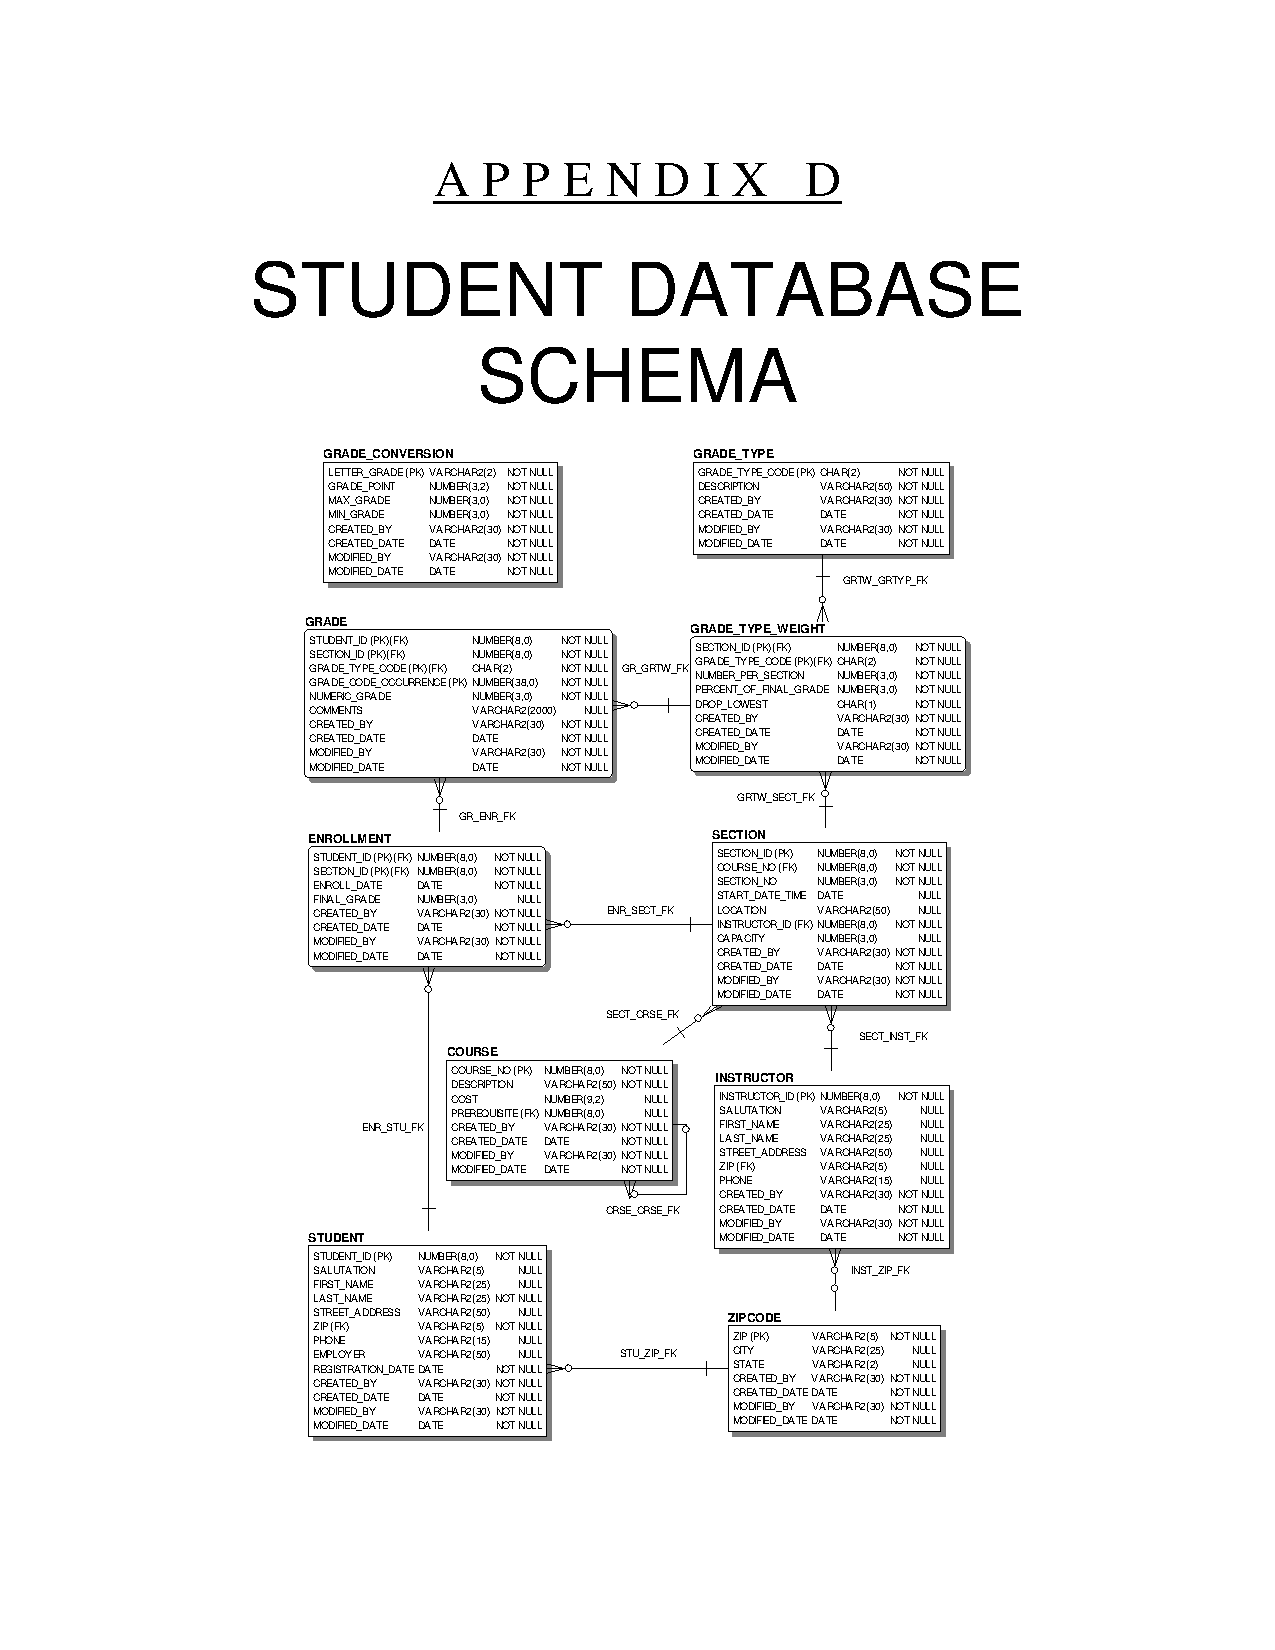
\includepdf{AppendixD.pdf}

\end{document}
